\chapter{Ambiente di sviluppo}

In questo capitolo saranno discusse le funzionalità e le possibilità offerte dal progetto in questione a favore del programmatore, nonché i vantaggi e le migliorie apportate nel processo di sviluppo.

La difficoltà principale che un programmatore si trova ad affrontare nell'intraprendere un percorso di apprendimento della programmazione embedded consiste nel ritrovarsi in un mondo completamente diverso di gestione del software e ambienti di sviluppo. Vi è poi l'assoluta differenza del processo di programmazione e debug da un comune applicativo per calcolatore.

Sebbene l'approccio a una nuova piattaforma hardware con differenti specifiche e funzionalità e, spesso, con un \textit{instruction set} limitato e non famigliare possa sembrare un ostacolo impegnativo, la verità è che, grazie a strumenti quali compilatori come \textit{gcc} e \textit{rustc}, è possibile scrivere notevoli porzioni di codice completamente indipendente dall'architettura del dispositivo finale.

La difficoltà principale per lo sviluppatore per approcciarsi allo sviluppo di una piattaforma embedded è di fatto l'adattarsi ad un nuovo ambiente e strumenti spesso proprietari e male o per nulla documentati.

Un'ulteriore difficoltà che limita l'accesso di nuovi sviluppatori verso il mondo embedded è la necessità di strumenti proprietari e costosi per programmare e \textit{debuggare} hardware, oltre al costo fisico di schede per la prototipazione.

Questi fattori sopra elencati hanno permesso alla società \textit{Arduino~s.r.l.} di entrare nel mercato dei dispositivi embedded mirando ad un pubblico inesperto e desideroso di approcciare una nuova pratica\cite{site:arduino-about}.

L'ecosistema Arduino è la scelta adottata dalla maggior parte di hobbisti e corsi di introduzione al mondo dell'elettronica digitale, motivati dalla dimensione della \textit{community}\footnote{Supporto di altri utenti fornito per mezzo di forum e mezzi anche non gestiti dall'azienda produttrice}, dal supporto, dagli strumenti sviluppati compatibili e semplici e dalla quantità di librerie \textit{open source} disponibili.

Non vi è dubbio sulla versatilità e la facilità di apprendimento della programmazione embedded AVR tramite la piattaforma.

Date le motivazioni e l'obiettivo dell'azienda d'Ivrea, è possibile osservare come la piattaforma e gli strumenti software con le loro  capacità non siano ottimali per uno sviluppo professionale o più complesso e ottimizzato: l'ambiente di sviluppo, mostrato in \cref{fig:arduino-ide}, è notevolmente semplificato causando una mancanza di strumenti essenziali.

\begin{figure}
    \centering
    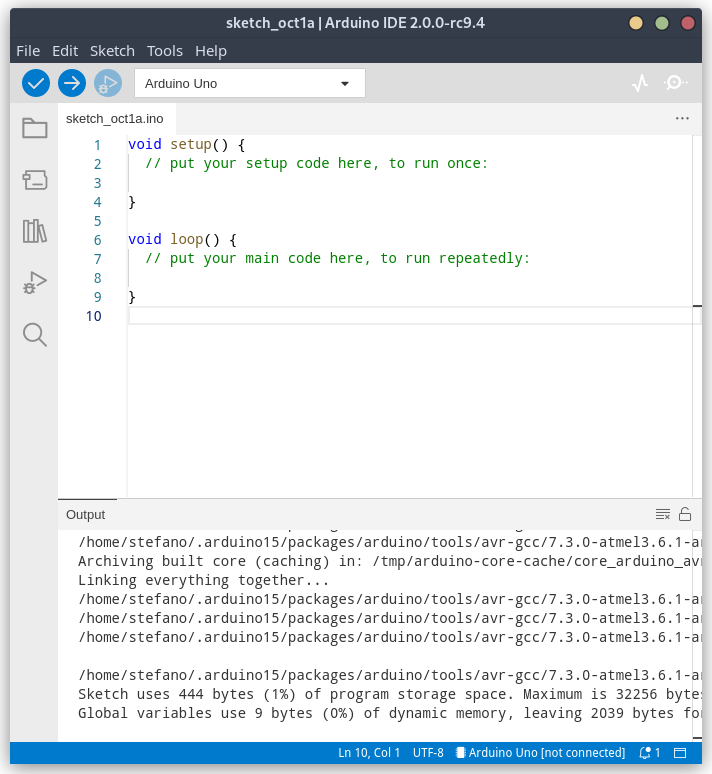
\includegraphics[width=.6\textwidth]{arduino-ide.png}
    \caption[Immagine di arduino IDE v2]{Finestra di programmazione dell'ambiente di sviluppo Arduino IDE v2}\label{fig:arduino-ide}
\end{figure}

Come è possibile osservare l'ambiente di sviluppo presenta un insieme notevolmente limitato di funzioni e un'interfaccia fortemente semplificata. È anche possibile osservare la presenza di un indicatore di debug: questo è solo disponibile con schede ARM a 32 bit più prestazionali. La funzionalità di debug non è presente sulle schede AVR.\@

Data l'assenza del \textit{debugger}, gli utenti sono obbligati all'utilizzo di logging tramite connessione seriale per analizzare il flusso del codice, pratica fortemente inefficiente per motivi prestazionali e per problemi di codifica dell'informazione.

L'utilizzo del server GDB sviluppato nel corso di questo elaborato garantirebbe nuove possibilità e efficienza, risultano però complesso e poco intuitivo in quanto dotato di sola interfaccia testuale come mostrato dalla~\cref{fig:gdb-cli}

\begin{figure}
    \centering
    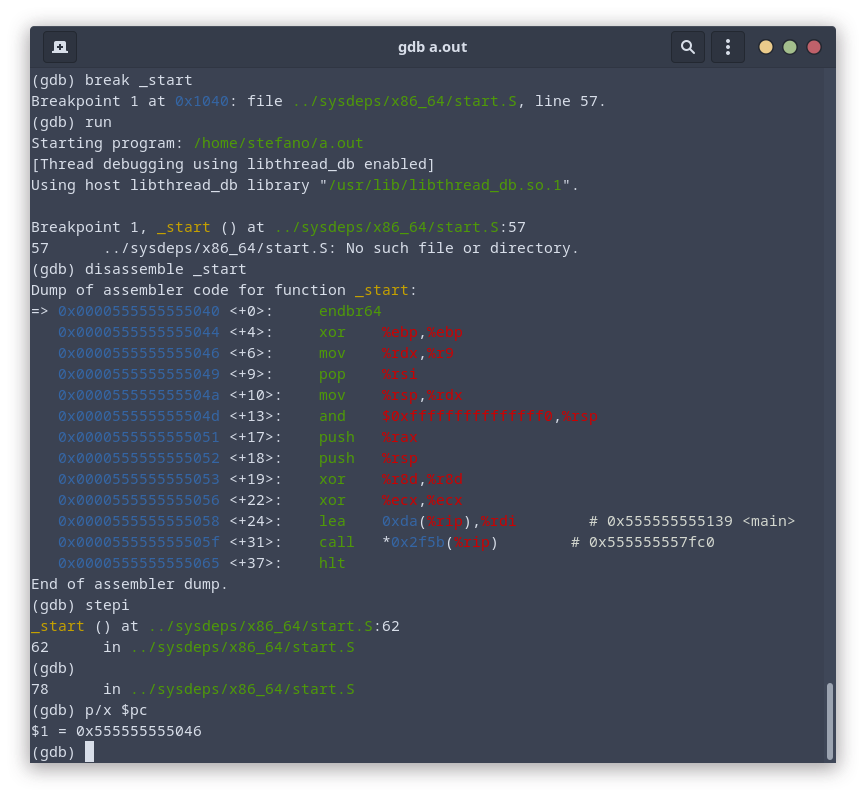
\includegraphics[width=.7\textwidth]{gdb-cli.png}
    \caption[]{Immagine di una sessione di debug da linea di comando}\label{fig:gdb-cli}
\end{figure}

Risulta quindi necessario sviluppare un insieme di componenti che possano essere integrate nella maggior parte degli ambienti di sviluppo senza difficoltà, permettendo così di superare una delle limitazioni sopra descritte, ovvero la difficoltà di adottare un ambiente di sviluppo nuovo e mal documentato, permettendo l'utilizzo di una piattaforma nota e configurabile.

\section{CMAKE}

Al fine di rendere la compilazione una procedura universale e generica è stato deciso l'utilizzo di un software di automazione del processo di compilazione altamente integrabile. Tale software è \textit{CMAKE}.

Esso permette di descrivere gli output della compilazione (obiettivi) e di impostare alcune variabili di configurazione per poi generare una procedura di compilazione in funzione dei pacchetti e delle caratteristiche disponibili sulla macchina, astraendo così dalla scrittura di codice interoperabile.

Inoltre, al fine di garantire interoperabilità tra ambienti di sviluppo, è stato deciso di affidare tutte le azioni di upload del codice a processi esterni che CMAKE permette di lanciare come degli obiettivi personalizzati.

L'integrazione con l'ambiente di sviluppo è invece affidata ad eventuali plugin per lo stesso o all'implementazione nativa del supporto per CMAKE.\@

Il~\cref{lst:cmake-target} mostra come un generico obiettivo di compilazione e programmazione viene descritto per poi essere tramutato in una procedura di compilazione.

È possibile notare come un singolo obiettivo per un dispositivo della piattaforma sia definito da tre distinti obiettivi concatenati e interdipendenti.

\noindent\begin{minipage}{\textwidth}
    \begin{lstlisting}[language=CMAKE, caption={Definizione di un target di compilazione e upload per un dispositivo AVR}, label=lst:cmake-target]
function(avrtarget targetName port)
    add_executable("${targetName}-elf" ${ARGN})
    target_link_options("${targetName}-elf" PUBLIC -Xlinker -T ${CMAKE_SOURCE_DIR}/cmake/linker/${MCU}.ld)
    add_custom_target(
        "${targetName}-bin" 
        COMMAND ${CMAKE_OBJCOPY} -O ihex -R .eeprom -R .fuse -R .lock -R .signature './${targetName}-elf' './${targetName}.hex';
        COMMAND ${CMAKE_OBJCOPY} -O ihex -j .eeprom './${targetName}-elf' './${targetName}.eeprom.hex';
        COMMAND ${CMAKE_SIZE} --mcu=${MCU} -C './${targetName}-elf';
        DEPENDS "${targetName}-elf"
    )
    add_custom_target(
        "${targetName}-upload"
        COMMAND python host_software/flash.py --port ${port} --flash './${targetName}.hex' --mcu ${MCU}
        USES_TERMINAL
        DEPENDS "${targetName}-bin"
    )
endfunction()

avrtarget(main main.c io.c)
target_link_libraries(main-elf rtt)
    \end{lstlisting}
\end{minipage}

In particolare sia \(main\) il nome generico assegnato al target avr in sviluppo. La procedura di compilazione generata da CMAKE conterrà tre target nominati
\begin{itemize}
    \item \textbf{main-elf}: obiettivo di compilazione effettivo dove il compilatore (\textit{avr-gcc}) verrà impiegato e genererà un file contenente codice eseguibile e informazioni di debug
    \item \textbf{main-bin}: obiettivo di utilità che estrarrà dal file \textit{build/main-elf} i file in formato \textit{ihex}\footnote{Intel Hexadecimal Format} per la programmazione delle memorie persistenti. Tali file sono una rappresentazione compressa del formato esadecimale\cite{site:ihex} e rappresentano le memorie bit per bit.
    \item \textbf{main-upload}: l'esecuzione di questo obiettivo esegue uno script che, dialogando con il server gdb, permette la scrittura della memoria flash e di conseguenza la programmazione senza uscire dalla modalità DebugWire.
\end{itemize}


